\section{Introduction}
\label{sec:introduction}

Systems for complex event processing (CEP)
continuously evaluate a set of
queries over streams of event
data~\cite{DBLP:journals/csur/CugolaM12,DBLP:journals/vldb/GiatrakosAADG20}.
 As such, they facilitate the
 analysis and anticipation of
situations of interest based on event patterns,
thereby enabling reactive and proactive
applications in various domains, including, for
instance, supply chain
management~\cite{DBLP:journals/cii/KonovalenkoL19},
 urban
transportation~\cite{DBLP:conf/edbt/ArtikisWSBLPBMKMGMGK14},
 and
computational
finance~\cite{DBLP:journals/computer/ChandramouliAGSR10}.

CEP systems provide a rich model for the
specification of
event queries~\cite{DBLP:conf/debs/ArtikisMUVW17}. Queries typically define
conditions over the attribute values of events to establish their relevance
for a pattern and to correlate them; and they impose constraints on the
ordering of events and their occurrence within a certain window over the
stream.

\update{}{
Queries to detect the event
patterns that are linked to a situation}
\update{M1\\M2\\M3\\R1O1}{of
interest enable predictive
applications~\cite{DBLP:conf/debs/EngelEF12,DBLP:conf/debs/SejdovicHRS16}. That
is, the occurrence of the situation may be anticipated in order to
to prevent or mitigate it. However, while domain experts may have
assumptions on the factors that
contribute to a
situation, the precise characterization of the respective event
patterns is difficult.}

\update{M2\\M4\\R1O1\\R2O1}{
For illustration purposes, consider a cluster monitoring scenario, in which events
denote state transitions of jobs~\cite{reiss2012towards}. For instance, in
\autoref{fig:overview}, the event $e_{11}$ would indicate that the job with ID $1$
has been \emph{scheduled} on the compute node producing the event stream $S_1$
with \emph{low} priority. A situation of interest
is the materialization of stragglers, i.e., nodes with comparatively large delays.
While a domain expert may understand that stragglers are linked to the
interference of jobs, the
specific execution patterns causing them are not known.}

\update{M1\\R1O1\\R2O1}{
Similar use cases are observed in
e.g., in urban transportation, where queries shall anticipate delays based on
events that represent
movements of
vehicles~\cite{DBLP:conf/edbt/ArtikisWSBLPBMKMGMGK14}.
 As another example, in computational
finance~\cite{DBLP:journals/computer/ChandramouliAGSR10},
 queries over events that denote
transactions and stock price changes help to
predict fraudulent behaviour.}

%\begin{wrapfigure}{r}{\columnwidth}
%	\centering
%	\vspace{-1em}
%
%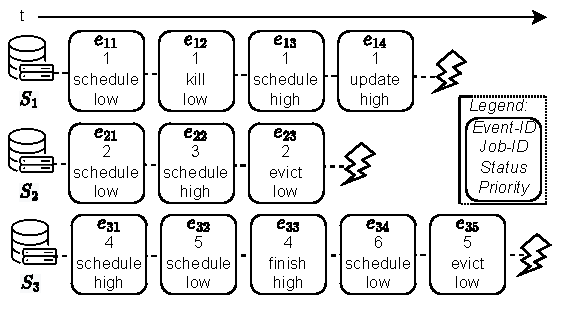
\includegraphics[width=0.9\columnwidth]{img/overview2.drawio.pdf}
%	\vspace{-2.0em}
%	\caption{todo.}
%	\label{fig:overview}
%	\vspace{-1em}
%\end{wrapfigure}
To support the specification of event queries, approaches for automated query
discovery have been proposed~\cite{icep,ilminer}. Given a database
of finite, historic (sub-)streams, each including at least one
materialization of
the situation, \update{M1\\M3\\R1O1\\R2O1}{they discover queries that match the
streams, thereby
generalizing the observations. Unlike machine learning approaches, the resulting
queries provide a traceable and
explainable characterization of the patterns that are correlated with the
situation of interest. They can be reviewed and refined by domain
experts, before they are used to anticipate (and potentially mitigate) the
respective situation in the
future, or to understand potential causes for
the situation based on the commonalities of the streams (similar to
discovering frequent item sets~\cite{DBLP:journals/widm/LunaFV19} or frequent
sequences~\cite{DBLP:journals/csur/MabroukehE10}).
}

\update{M4\\R1O1\\R2O1}{
In our example in \autoref{fig:overview}, for instance, streams of three
nodes that became stragglers in the past are given. For this setting, queries that
characterize common event patterns are discovered. The
example shows a query in SASE notation~\cite{DBLP:conf/sigmod/ZhangDI14}, in which
scheduling of a low-priority job is followed by an event of a high-priority
job (on the same node), before another event occurs for the first job.}


Solving the problem of event query discovery is computationally hard, though.
The search space of candidate queries grows exponentially in
the query length and the size of the domain of the payload data. Existing
discovery approaches~\cite{icep,ilminer} explore this
space in \emph{one} specific way, which may be suitable for one
database, but leads to intractability for another one. Yet, the assumptions on
the database that motivate the taken design choices are implicit, so that it is
unclear for which database an algorithm can be expected to work.


In this paper, we take up the general idea of event query discovery, and aim at
answering the following questions:
\begin{enumerate}[label=(\roman*),left=0pt,nosep]
\item \emph{What are the design choices in query discovery?}
\item \emph{How to choose a design for a given database?}
\item \emph{How to provide feedback on the algorithmic performance?}
\end{enumerate}
\update{M5\\R3O1}{By addressing these questions, we provide a conceptual
foundation to
study solutions to the problem of event query discovery. For the first time, this
enables a systematic description and realization of the various algorithmic design
choices, and outlines their implications in the practical use of discovery
algorithms for a given stream database.} Specifically, our contributions and the
paper structure following a problem formalization
(\autoref{sec:problem}), are summarized as follows:
\begin{enumerate}[left=0pt,nosep]
\item We present \sys{} (\autoref{sec:framework})
as a framework
for the design of algorithms for event query
discovery. It captures a set of fundamental design
choices to define discovery algorithms.
\item We instantiate the framework to derive four
discovery algorithms
(\autoref{sec:algos}). They all provide correct
and complete results, yet they differ in their exploration of the space of
candidate queries.
\item We provide means to guide event query discovery
(\autoref{sec:instantiation}). First, we show how to choose among our
algorithms based on a few essential properties of a given stream database.
Second, we provide hints on how to resolve intractability or ineffectiveness of
discovery based on abstractions of the events' payload data.
\end{enumerate}
We evaluated the algorithms devised within the \sys{} framework in experiments
using simulated
and real-world data (\autoref{sec:evaluation}).
\update{}{Our results} \update{M5\\R3O1}{highlight that our algorithms are more
effective and
more efficient than the state of
the art.
We discover more expressive queries and solve
the discovery problem
several orders of magnitude faster than existing, complete approaches;
with runtimes that are comparable to
strategies that approximate the result.
Moreover, we show that our algorithms are indeed tailored to databases
that show certain properties, thereby providing insights into the practical
applicability of our techniques.}
Finally, we review related work (\autoref{sec:related_work}) and
conclude~(\autoref{sec:conclusions}).


\begin{figure}[t]
	\centering
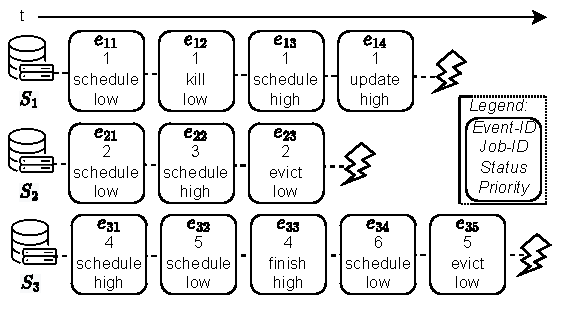
\includegraphics[width=0.82\columnwidth]{img/overview2.drawio.pdf}
\vspace{-.5em}
\begin{flushleft}
{\footnotesize
\begin{verbatim}
PATTERN SEQ (E e1, E e2, E e3)
WHERE e1.Job-ID = e3.Job-ID AND e1.Status = schedule
AND e1.Priority = low AND e2.Priority = high
\end{verbatim}
}
\end{flushleft}
	\vspace{-1em}
	\caption{
	\update{{\normalfont M4\\R1O1\\R2O1}}{Three streams emitted by nodes in a
	compute
	cluster. Each event
	carries an identifier (e.g., $e_{11}$), a job ID (e.g., $1$), a state
	transition (e.g., \emph{schedule}), and a priority (e.g., \emph{low}). A query
	in SASE notation~\cite{DBLP:conf/sigmod/ZhangDI14} defines a pattern over the
	streams.}}
	\label{fig:overview}
	\vspace{-1.5em}
\end{figure}
